% =============================================
% CAPÍTULO 4: PRUEBAS Y RESULTADOS
% =============================================

\chapterpage{4}{Pruebas y Resultados}
\clearpage
\refstepcounter{chapter}
\addcontentsline{toc}{chapter}{Cap. 4 Pruebas y Resultados}

En este capítulo se documentan las pruebas realizadas sobre cada componente del sistema construido en el capítulo anterior y los resultados obtenidos. Las pruebas se presentan siguiendo el mismo orden de los objetivos específicos: base de datos, API REST, interfaz web y nodo sensor. Para cada componente se describen los escenarios verificados, los ajustes que fue necesario realizar a partir de los resultados obtenidos, y las mejoras identificadas durante el proceso de validación.

% =============================================
% SECCIÓN 4.1: BASE DE DATOS
% =============================================

\section{Pruebas de la base de datos}

La base de datos no se probó de forma aislada sino a través de la suite de pruebas automatizadas de la API: dado que cada prueba opera sobre una instancia real de PostgreSQL, cualquier restricción, índice o relación que no funcione correctamente provoca un fallo detectable en la prueba correspondiente. Este enfoque permitió validar el comportamiento de la base de datos en las mismas condiciones que en producción, sin necesidad de escribir pruebas separadas a nivel de base de datos.

\subsection{Restricciones e integridad relacional}

Las restricciones definidas en el esquema —claves foráneas, unicidad y valores no nulos— se verificaron a través de los casos de prueba negativos de la API: intentar crear un lote con un producto inexistente devuelve error, intentar registrar un usuario con un correo ya registrado devuelve error, e intentar completar una venta vacía es rechazado por el sistema. En todos los casos el motor de base de datos aplicó la restricción correspondiente y la API tradujo ese rechazo en un código de respuesta apropiado.

Un caso de diseño particular que se verificó fue el de los lotes sin número de código asignado. El inventario permite que un lote no tenga código —situación que ocurre cuando el fabricante no imprime uno— pero si un código está presente, no puede repetirse para el mismo producto. Para implementar esto sin bloquear los lotes sin código se utilizó un índice parcial: la restricción de unicidad aplica únicamente cuando el campo tiene un valor, ignorando los registros en que está vacío. La figura siguiente ilustra cómo se comporta este índice en la práctica:

\begin{figure}[H]
\centering
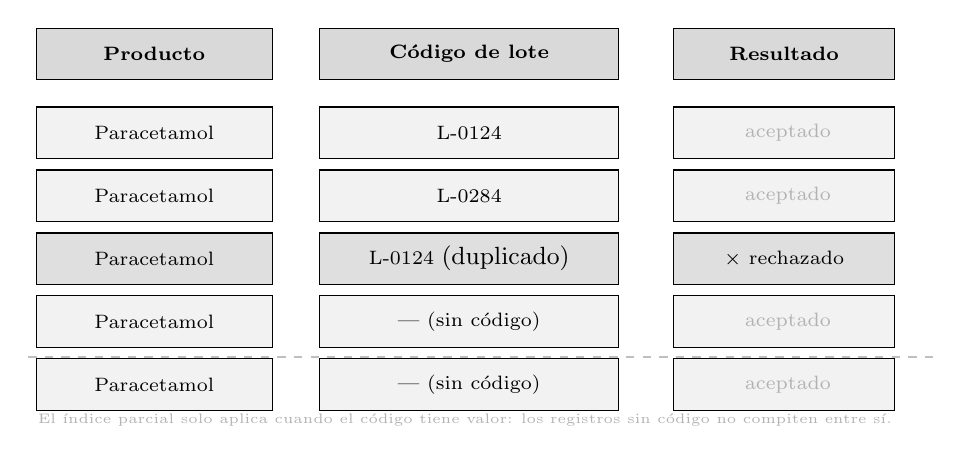
\begin{tikzpicture}[font=\small,
    row/.style={rectangle, draw, minimum width=3.8cm, minimum height=0.65cm,
                align=center, font=\scriptsize},
    ok/.style={row, fill=gray!10},
    bad/.style={row, fill=gray!25}
]

% ── Columnas header ───────────────────────────────────────────
\node[row, fill=gray!30, minimum width=3.0cm] (h1) at (0,    4.2) {\textbf{Producto}};
\node[row, fill=gray!30, minimum width=3.8cm] (h2) at (4.0,  4.2) {\textbf{Código de lote}};
\node[row, fill=gray!30, minimum width=2.8cm] (h3) at (8.0,  4.2) {\textbf{Resultado}};

% ── Caso 1: lote con código único → aceptado ─────────────────
\node[ok, minimum width=3.0cm] at (0,   3.2) {Paracetamol};
\node[ok, minimum width=3.8cm] at (4.0, 3.2) {L-0124};
\node[ok, minimum width=2.8cm, text=gray!60] at (8.0, 3.2) {\checkmark\ aceptado};

% ── Caso 2: segundo lote del mismo producto, código diferente → aceptado
\node[ok, minimum width=3.0cm] at (0,   2.4) {Paracetamol};
\node[ok, minimum width=3.8cm] at (4.0, 2.4) {L-0284};
\node[ok, minimum width=2.8cm, text=gray!60] at (8.0, 2.4) {\checkmark\ aceptado};

% ── Caso 3: código duplicado para el mismo producto → rechazado
\node[bad, minimum width=3.0cm] at (0,   1.6) {Paracetamol};
\node[bad, minimum width=3.8cm] at (4.0, 1.6) {L-0124 \small(duplicado)};
\node[bad, minimum width=2.8cm] at (8.0, 1.6) {$\times$\ rechazado};

% ── Caso 4: lote sin código, mismo producto → aceptado (índice parcial)
\node[ok, minimum width=3.0cm] at (0,   0.8) {Paracetamol};
\node[ok, minimum width=3.8cm] at (4.0, 0.8) {— (sin código)};
\node[ok, minimum width=2.8cm, text=gray!60] at (8.0, 0.8) {\checkmark\ aceptado};

% ── Caso 5: segundo lote sin código, mismo producto → también aceptado
\node[ok, minimum width=3.0cm] at (0,   0.0) {Paracetamol};
\node[ok, minimum width=3.8cm] at (4.0, 0.0) {— (sin código)};
\node[ok, minimum width=2.8cm, text=gray!60] at (8.0, 0.0) {\checkmark\ aceptado};

% ── Nota explicativa ──────────────────────────────────────────
\draw[dashed, gray!50] (-1.6, 0.35) -- (9.9, 0.35);
\node[anchor=west, font=\tiny, text=gray!60] at (-1.6, -0.45)
    {El índice parcial solo aplica cuando el código tiene valor: los registros sin código no compiten entre sí.};

\end{tikzpicture}
\caption{Comportamiento del índice parcial sobre el código de lote: los códigos duplicados son rechazados, pero múltiples lotes sin código del mismo producto son permitidos}
\label{fig:cap4-lote-index}
\vspace{0.2cm}
\footnotesize \textbf{Fuente:} Elaboración propia.
\end{figure}

\subsection{Ajustes al esquema durante el desarrollo}

El diseño inicial de la base de datos descrito en el capítulo anterior continuó evolucionando durante la implementación. A medida que se desarrollaban los módulos de la API y se ejecutaban las pruebas, se identificaron aspectos del esquema que requerían ajuste. Estos cambios se aplicaron mediante migraciones sucesivas que modifican la estructura de la base de datos de forma controlada, preservando los datos existentes. La tabla siguiente resume los ajustes más relevantes:

\begin{longtable}{|p{4.0cm}|p{10.5cm}|}

\caption{Ajustes al esquema de la base de datos durante el desarrollo} \label{tab:cap4-migraciones} \\

\hline
\rowcolor{gray!20}
\textbf{Ajuste} & \textbf{Motivo} \\
\hline
\endfirsthead

\hline
\rowcolor{gray!20}
\textbf{Ajuste} & \textbf{Motivo} \\
\hline
\endhead

\hline
\multicolumn{2}{|r|}{\small Continúa en la siguiente página} \\
\hline
\endfoot

\hline
\endlastfoot

Tipo de dato para montos monetarios &
Las columnas de precio, subtotal y total se definieron inicialmente como números de punto flotante. Al realizar cálculos con precios decimales los totales acumulaban errores de redondeo. Se migró a tipo de dato de precisión decimal exacta, que garantiza resultados exactos independientemente del número de operaciones. \\
\hline

Borrado lógico en tablas clave &
Se añadió una columna de fecha de baja a las tablas de usuarios, roles, sucursales y productos. Esto permite desactivar registros sin eliminarlos, preservando el historial de ventas y el vínculo con el usuario que realizó cada transacción. \\
\hline

Índice parcial sobre código de lote &
Para permitir que un lote no tenga código asignado —situación habitual con algunos proveedores— sin perder la garantía de que los códigos presentes no se dupliquen, se reemplazó la restricción de unicidad simple por un índice que aplica únicamente cuando el campo tiene valor. \\
\hline

Tipos enumerados nativos de PostgreSQL &
Los estados de ventas, pagos, género y tipo de documento se definieron inicialmente como texto libre. Al migrar a tipos enumerados nativos del motor de base de datos, el propio motor rechaza valores no permitidos y la búsqueda sobre esos campos se vuelve más eficiente. \\
\hline

Índices sobre claves foráneas &
Se identificó durante las pruebas que las consultas con combinaciones de tablas —como obtener un lote con su producto asociado— resultaban lentas sin índices en las columnas de referencia. Se añadieron índices en las claves foráneas de las tablas de mayor uso. \\
\hline

Restricciones únicas en proveedor &
Las restricciones de unicidad sobre el RFC y correo electrónico del proveedor impedían reutilizar esos datos al dar de baja y reactivar un proveedor. La validación se trasladó al código de la API, eliminando la restricción del esquema. \\

\end{longtable}
\vspace{0.1cm}
{\footnotesize \textbf{Fuente:} Elaboración propia.}

% TODO: insertar captura de pantalla del diagrama de la base de datos en DataGrip o similar
% (el diagrama general del esquema con las 22 tablas y sus relaciones)
% Guardar en: 0_imagenes/Cap4/EsquemaBD.png
%\begin{figure}[H]
%    \centering
%    \fbox{\includegraphics[width=\textwidth]{0_imagenes/Cap4/EsquemaBD.png}}
%    \caption{Esquema final de la base de datos con las 22 tablas y sus relaciones}
%    \label{fig:cap4-esquema-bd}
%    \vspace{0.2cm}
%    \footnotesize \textbf{Fuente:} Elaboración propia.
%\end{figure}

\subsection{Resultados}

El esquema final de la base de datos opera de forma estable en el entorno de producción de Railway. Todas las restricciones verificadas —integridad referencial, unicidad condicional, borrado lógico y precisión monetaria— funcionan de forma correcta bajo la carga de las pruebas automatizadas. Los seis ajustes documentados en la tabla anterior resolvieron los comportamientos incorrectos identificados durante el desarrollo y no requirieron modificaciones adicionales tras su aplicación.

% =============================================
% SECCIÓN 4.2: API REST
% =============================================

\clearpage
\section{Pruebas de la API REST}

Para verificar el funcionamiento de la API se desarrolló una suite de pruebas automatizadas que cubre la totalidad de los módulos del sistema. Cada prueba opera sobre una base de datos PostgreSQL real en lugar de datos simulados, lo que garantiza que el comportamiento verificado sea idéntico al que se ejecuta en producción: una prueba sobre datos simulados puede pasar aunque el sistema real falle, mientras que una prueba sobre la base de datos real detecta ese tipo de diferencias. La suite abarca escenarios positivos —operaciones que deben completarse con éxito— y negativos —operaciones que el sistema debe rechazar—, y cubre los módulos de autenticación, usuarios, roles, productos, inventario, ventas, compras, proveedores y sensor.

Las pruebas se ejecutaron primero en el entorno local de desarrollo y posteriormente en un entorno de integración continua que las corre de forma automática con cada actualización del código.

\subsection{Módulo de autenticación}

Con la implementación inicial del módulo de autenticación se obtuvo un sistema que emitía un token de acceso al iniciar sesión y lo verificaba en cada operación posterior. Durante las pruebas se identificó que el tiempo de vigencia del token resultaba insuficiente para sesiones de trabajo prolongadas: el sistema cerraba la sesión del usuario mientras este se encontraba operando la aplicación, lo que interrumpía el flujo de trabajo.

Para resolver este comportamiento fue necesario incorporar un segundo token de mayor duración, denominado token de refresco. El token de acceso mantiene su vigencia de 30 minutos para las operaciones regulares; cuando está próximo a expirar, el sistema lo renueva de forma transparente sin que el usuario tenga que iniciar sesión nuevamente. Se añadió además la opción de sesión prolongada —equivalente a la función \textit{recordarme} en aplicaciones web— que extiende la duración del token de refresco a 30 días para los usuarios que así lo seleccionen al iniciar sesión.

% TODO: insertar captura de pantalla de la pantalla de inicio de sesión mostrando la opción "Recordarme"
% Guardar en: 0_imagenes/Cap4/LoginRecordarme.png
%\begin{figure}[H]
%    \centering
%    \fbox{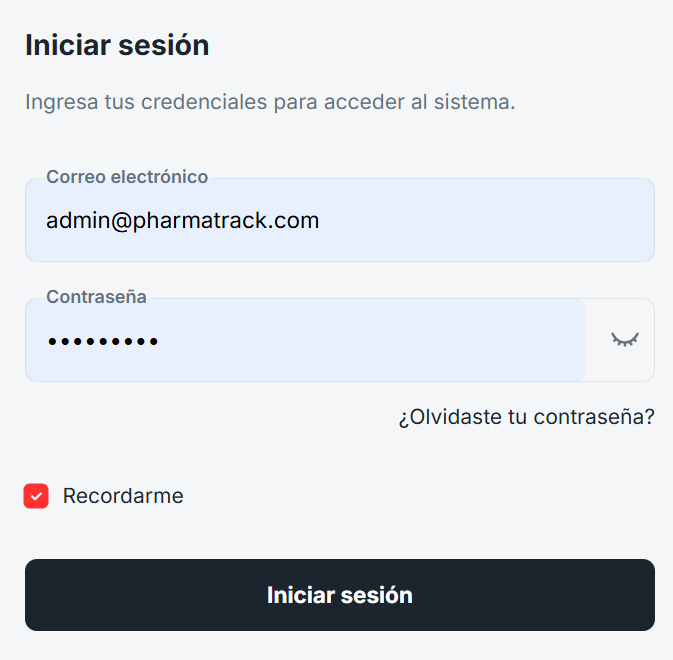
\includegraphics[width=0.65\textwidth]{0_imagenes/Cap4/LoginRecordarme.png}}
%    \caption{Pantalla de inicio de sesión con la opción de sesión prolongada}
%    \label{fig:cap4-login}
%    \vspace{0.2cm}
%    \footnotesize \textbf{Fuente:} Elaboración propia.
%\end{figure}

\begin{figure}[H]
\centering
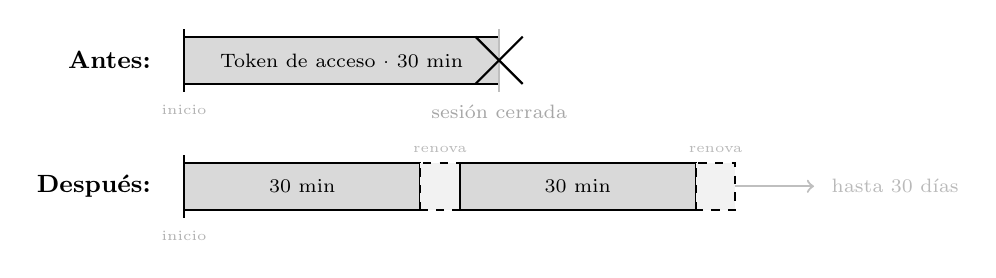
\begin{tikzpicture}[font=\small]

% ── Etiquetas de fila ─────────────────────────────────────────
\node[anchor=east, font=\small\bfseries] at (-0.3,  1.0) {Antes:};
\node[anchor=east, font=\small\bfseries] at (-0.3, -0.6) {Después:};

% ── ANTES: token único que expira y cierra la sesión ──────────
\fill[gray!30] (0, 0.7) rectangle (4.0, 1.3);
\draw[thick]   (0, 0.7) rectangle (4.0, 1.3);
\node[font=\scriptsize] at (2.0, 1.0) {Token de acceso · 30 min};
% marca de inicio
\draw[thick] (0, 0.6) -- (0, 1.4);
\node[anchor=north, font=\tiny, text=gray!60] at (0, 0.55) {inicio};
% marca de expiración
\draw[thick, gray!50] (4.0, 0.6) -- (4.0, 1.4);
\draw[thick] (3.7, 0.7) -- (4.3, 1.3);
\draw[thick] (4.3, 0.7) -- (3.7, 1.3);
\node[anchor=north, font=\scriptsize, text=gray!70] at (4.0, 0.55)
    {sesión cerrada};

% ── DESPUÉS: access token + renovación silenciosa ─────────────
% token 1
\fill[gray!30] (0, -0.9) rectangle (3.0, -0.3);
\draw[thick]   (0, -0.9) rectangle (3.0, -0.3);
\node[font=\scriptsize] at (1.5, -0.6) {30 min};
% renovación 1
\fill[gray!10] (3.0, -0.9) rectangle (3.5, -0.3);
\draw[thick, dashed] (3.0, -0.9) rectangle (3.5, -0.3);
\node[anchor=south, font=\tiny, text=gray!55] at (3.25, -0.3)
    {renova};
% token 2
\fill[gray!30] (3.5, -0.9) rectangle (6.5, -0.3);
\draw[thick]   (3.5, -0.9) rectangle (6.5, -0.3);
\node[font=\scriptsize] at (5.0, -0.6) {30 min};
% renovación 2
\fill[gray!10] (6.5, -0.9) rectangle (7.0, -0.3);
\draw[thick, dashed] (6.5, -0.9) rectangle (7.0, -0.3);
\node[anchor=south, font=\tiny, text=gray!55] at (6.75, -0.3)
    {renova};
% continúa
\draw[->, thick, gray!50] (7.0, -0.6) -- (8.0, -0.6);
\node[anchor=west, font=\scriptsize, text=gray!55] at (8.1, -0.6)
    {hasta 30 días};
% marca de inicio
\draw[thick] (0, -1.0) -- (0, -0.2);
\node[anchor=north, font=\tiny, text=gray!60] at (0, -1.05) {inicio};

\end{tikzpicture}
\caption{Evolución del sistema de sesión: la versión inicial cerraba la sesión al expirar el token de acceso; la versión final lo renueva de forma automática y transparente para el usuario}
\label{fig:cap4-token-timeline}
\vspace{0.2cm}
\footnotesize \textbf{Fuente:} Elaboración propia.
\end{figure}

Durante las pruebas también se identificó que el módulo de cambio de contraseña no verificaba que el usuario con sesión activa fuera el mismo que intentaba realizar el cambio, lo que representaba una vulnerabilidad: un usuario podría haber modificado la contraseña de otro. Esta situación se corrigió añadiendo una verificación de identidad antes de procesar la solicitud.

\subsection{Módulo de ventas y control de inventario por lotes}

La lógica de completar una venta —que descuenta las unidades vendidas del inventario y registra de qué lote provienen— fue el componente de mayor complejidad de la API. Con la propuesta inicial del registro de ventas se contaba únicamente con el encabezado de la transacción y el detalle de los productos; el descuento efectivo del inventario por lote no estaba implementado en esa versión.

Para cubrir este comportamiento fue necesario desarrollar un módulo adicional que implementa la política FEFO (\textit{First Expired, First Out}: primero en vencer, primero en salir). Al confirmar una venta, el sistema identifica los lotes disponibles del producto vendido, los ordena por fecha de caducidad y descuenta las unidades del lote que vence primero. Si las existencias de un lote no son suficientes para cubrir la cantidad vendida, el sistema distribuye automáticamente el descuento entre los lotes siguientes en orden de caducidad. Este comportamiento se verificó con pruebas que cubren los casos: descuento completo desde un único lote, distribución entre múltiples lotes, e intento de venta con existencias insuficientes —en este último caso el sistema rechaza la operación y el inventario no se ve afectado.

\begin{figure}[H]
\centering
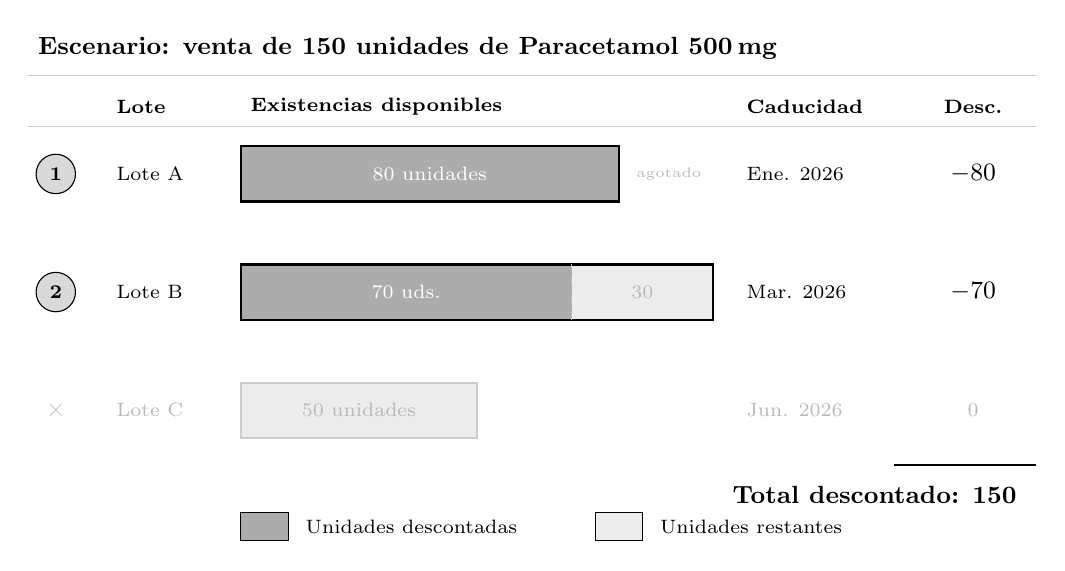
\begin{tikzpicture}[font=\small]

% ── Encabezado ────────────────────────────────────────────────
\node[anchor=west, font=\small\bfseries] at (0.0, 5.5)
    {Escenario: venta de 150 unidades de Paracetamol 500\,mg};
\draw[gray!40] (0.0, 5.15) -- (12.8, 5.15);

% ── Cabeceras de columna ──────────────────────────────────────
\node[anchor=west, font=\scriptsize\bfseries] at (1.0, 4.75) {Lote};
\node[anchor=west, font=\scriptsize\bfseries] at (2.7, 4.75) {Existencias disponibles};
\node[anchor=west, font=\scriptsize\bfseries] at (9.0, 4.75) {Caducidad};
\node[anchor=center,font=\scriptsize\bfseries] at (12.0, 4.75) {Desc.};
\draw[gray!40] (0.0, 4.50) -- (12.8, 4.50);

% ── Lote A (80 uds, completamente consumido) ─────────────────
% orden
\node[circle, draw, fill=gray!30, minimum size=0.5cm,
      inner sep=0pt, font=\scriptsize\bfseries] at (0.35, 3.9) {1};
\node[anchor=west, font=\scriptsize] at (1.0, 3.9) {Lote A};
% barra: escala 0.06 cm/ud → 80 uds = 4.80 cm desde x=2.7
\fill[gray!65] (2.7, 3.55) rectangle (7.50, 4.25);
\draw[thick]   (2.7, 3.55) rectangle (7.50, 4.25);
\node[font=\scriptsize, text=white] at (5.10, 3.90) {80 unidades};
\node[anchor=west, font=\scriptsize] at (9.0, 3.90) {Ene. 2026};
\node[anchor=center, font=\small\bfseries] at (12.0, 3.90) {$-80$};
% etiqueta agotado
\node[anchor=west, font=\tiny, text=gray!55] at (7.60, 3.90) {agotado};

% ── Lote B (100 uds, 70 consumidas) ──────────────────────────
\node[circle, draw, fill=gray!30, minimum size=0.5cm,
      inner sep=0pt, font=\scriptsize\bfseries] at (0.35, 2.4) {2};
\node[anchor=west, font=\scriptsize] at (1.0, 2.4) {Lote B};
% barra total: 100 uds = 6.00 cm → x=2.7..8.70
% consumido: 70 uds = 4.20 cm → x=2.7..6.90
% restante:  30 uds = 1.80 cm → x=6.90..8.70
\fill[gray!65] (2.7, 2.05) rectangle (6.90, 2.75);
\fill[gray!15] (6.9, 2.05) rectangle (8.70, 2.75);
\draw[thick]   (2.7, 2.05) rectangle (8.70, 2.75);
\draw[dashed, gray!50] (6.9, 2.05) -- (6.9, 2.75);
\node[font=\scriptsize, text=white]    at (4.80, 2.40) {70 uds.};
\node[font=\scriptsize, text=gray!55]  at (7.80, 2.40) {30};
\node[anchor=west, font=\scriptsize]   at (9.0,  2.40) {Mar. 2026};
\node[anchor=center, font=\small\bfseries] at (12.0, 2.40) {$-70$};

% ── Lote C (50 uds, sin tocar) ───────────────────────────────
\node[font=\small, text=gray!45] at (0.35, 0.9) {$\times$};
\node[anchor=west, font=\scriptsize, text=gray!55] at (1.0, 0.9) {Lote C};
% barra: 50 uds = 3.00 cm → x=2.7..5.70, sin consumo
\fill[gray!15]     (2.7, 0.55) rectangle (5.70, 1.25);
\draw[thick, gray!40] (2.7, 0.55) rectangle (5.70, 1.25);
\node[font=\scriptsize, text=gray!55] at (4.20, 0.90) {50 unidades};
\node[anchor=west, font=\scriptsize, text=gray!55] at (9.0, 0.90) {Jun. 2026};
\node[anchor=center, font=\scriptsize, text=gray!55] at (12.0, 0.90) {$0$};

% ── Separador y total ─────────────────────────────────────────
\draw[thick] (11.0, 0.20) -- (12.8, 0.20);
\node[anchor=east, font=\small\bfseries] at (12.8, -0.18)
    {Total descontado: 150 $\checkmark$};

% ── Leyenda ───────────────────────────────────────────────────
\fill[gray!65] (2.7, -0.75) rectangle (3.30, -0.40);
\draw          (2.7, -0.75) rectangle (3.30, -0.40);
\node[anchor=west, font=\scriptsize] at (3.40, -0.58) {Unidades descontadas};
\fill[gray!15] (7.2, -0.75) rectangle (7.80, -0.40);
\draw          (7.2, -0.75) rectangle (7.80, -0.40);
\node[anchor=west, font=\scriptsize] at (7.90, -0.58) {Unidades restantes};

\end{tikzpicture}
\caption{Ejemplo de la política FEFO aplicada en el módulo de ventas: el sistema consume primero el lote con la caducidad más próxima; si sus existencias no alcanzan, continúa con el siguiente lote en orden}
\label{fig:cap4-fefo}
\vspace{0.2cm}
\footnotesize \textbf{Fuente:} Elaboración propia.
\end{figure}

Junto con la lógica de ventas se implementó y verificó el módulo de devoluciones. Una devolución revierte el descuento de inventario aplicado al completar la venta, reintegrando las unidades a los mismos lotes de los que fueron descontadas. El estado de la venta se actualiza automáticamente a \textit{parcialmente devuelta} o \textit{devuelta} según la cantidad retornada, sin intervención manual.

\subsection{Correcciones identificadas durante las pruebas}

A lo largo del proceso de verificación se identificaron y corrigieron problemas en distintos módulos de la API. La tabla siguiente resume los más representativos:

\begin{longtable}{|p{3.0cm}|p{4.2cm}|p{7.3cm}|}

\caption{Correcciones realizadas a la API durante las pruebas} \label{tab:cap4-api-correcciones} \\

\hline
\rowcolor{gray!20}
\textbf{Módulo} & \textbf{Problema identificado} & \textbf{Corrección aplicada} \\
\hline
\endfirsthead

\hline
\rowcolor{gray!20}
\textbf{Módulo} & \textbf{Problema identificado} & \textbf{Corrección aplicada} \\
\hline
\endhead

\hline
\multicolumn{3}{|r|}{\small Continúa en la siguiente página} \\
\hline
\endfoot

\hline
\endlastfoot

Cálculos monetarios &
Los totales de ventas acumulaban errores de redondeo al operar con precios decimales &
Se cambió el tipo de dato de las columnas de monto a precisión decimal exacta, eliminando los errores de redondeo \\
\hline

Registros dados de baja &
Los registros eliminados seguían apareciendo en los listados de búsqueda y consulta &
Se añadió el filtro correspondiente en todas las consultas de lectura del sistema \\
\hline

Comunicación con el navegador &
Los errores internos del servidor llegaban al navegador como errores de red genéricos, sin mensaje descriptivo &
Se ajustó la configuración para que todos los tipos de respuesta, incluyendo los errores, incluyeran las cabeceras de acceso necesarias \\
\hline

Despliegue en Railway &
El servidor de producción no encontraba el módulo de la aplicación al iniciar, impidiendo el arranque &
Se corrigió la ruta de inicio en el archivo de configuración del servidor en Railway \\
\hline

Búsqueda de usuarios &
La búsqueda por tipo de documento no funcionaba porque el motor de base de datos no permite búsqueda parcial sobre campos de tipo enumerado &
Se modificó la consulta para convertir el campo a texto antes de aplicar el filtro de búsqueda \\
\hline

Recuperación de contraseña &
El servicio externo de envío de correo cambió su interfaz entre versiones, interrumpiendo el flujo de recuperación &
Se actualizó la integración con la nueva versión del servicio \\

\end{longtable}
\vspace{0.1cm}
{\footnotesize \textbf{Fuente:} Elaboración propia.}

\subsection{Resultados de la suite de pruebas}

La suite de pruebas cubre los veinte módulos de la API con casos por operación: lectura, creación, actualización y eliminación, más los escenarios de rechazo para cada uno —solicitudes sin autenticación, identificadores inexistentes y datos con formato incorrecto. Todos los casos de prueba pasan de forma exitosa sobre la base de datos de producción en Railway, lo que confirma que el comportamiento del sistema es consistente con el diseño descrito en el capítulo anterior.

% TODO: insertar captura de pantalla de la terminal mostrando los tests pasando (salida de pytest)
% Guardar en: 0_imagenes/Cap4/PytestResultados.png
%\begin{figure}[H]
%    \centering
%    \fbox{\includegraphics[width=0.85\textwidth]{0_imagenes/Cap4/PytestResultados.png}}
%    \caption{Resultado de la ejecución de la suite de pruebas automatizadas de la API}
%    \label{fig:cap4-pytest}
%    \vspace{0.2cm}
%    \footnotesize \textbf{Fuente:} Elaboración propia.
%\end{figure}

% =============================================
% SECCIÓN 4.3: FRONTEND REACT
% =============================================

\clearpage
\section{Pruebas de la interfaz web}

La verificación de la interfaz web se realizó de forma iterativa a lo largo del desarrollo: cada módulo se probó manualmente en el navegador al momento de construirse, conectándolo contra la API desplegada en Railway para verificar que los datos fluyeran correctamente de extremo a extremo. De forma complementaria, se desarrolló un conjunto de pruebas automatizadas para los componentes individuales de mayor criticidad.

La figura siguiente muestra el flujo general de navegación: desde el inicio de sesión hasta el registro de una venta, con los módulos adicionales accesibles desde el menú lateral de la aplicación.

% ─────────────────────────────────────────────────────────────────────────
% WIREFLOW DE NAVEGACIÓN
% Cuando tengas capturas reales, en cada nodo reemplaza el \parbox por:
%   \includegraphics[width=Xcm,height=2.4cm]{0_imagenes/Cap4/NombreArchivo.png}
% ─────────────────────────────────────────────────────────────────────────
\begin{figure}[H]
\centering
\resizebox{\linewidth}{!}{%
\begin{tikzpicture}[
  screen/.style={
    rectangle split, rectangle split parts=2,
    rectangle split part fill={gray!25, white},
    draw=gray!55, thick, rounded corners=3pt,
    minimum width=4cm, text width=3.8cm,
    align=center, inner sep=4pt
  },
  hub/.style={
    rectangle split, rectangle split parts=2,
    rectangle split part fill={gray!60, gray!8},
    draw=black!75, very thick, rounded corners=3pt,
    minimum width=4.2cm, text width=4.0cm,
    align=center, inner sep=4pt
  },
  mainArrow/.style={->, >=Stealth, line width=1.4pt, draw=black!65},
  branchArrow/.style={->, >=Stealth, line width=0.9pt, draw=gray!60, dashed},
  lbl/.style={font=\tiny\sffamily, text=black!60, fill=white, inner sep=1.5pt}
]

% ── FILA PRINCIPAL (flujo de registro de venta) ──────────────────────

% 1. Login
% TODO: reemplazar parbox por 
\includegraphics[width=3.8cm,height=2.4cm]{0_imagenes/Cap4/Login.png}
\node[screen] (login) at (0, 0) {%
  \textbf{\scriptsize Inicio de sesión}%
  \nodepart{two}%
  \parbox[c][2.4cm][c]{3.8cm}{\centering\textcolor{gray!50}{\small\itshape [Login.png]}}%
};

% 2. Dashboard (nodo hub — punto de acceso a todos los módulos)
% TODO: reemplazar parbox por 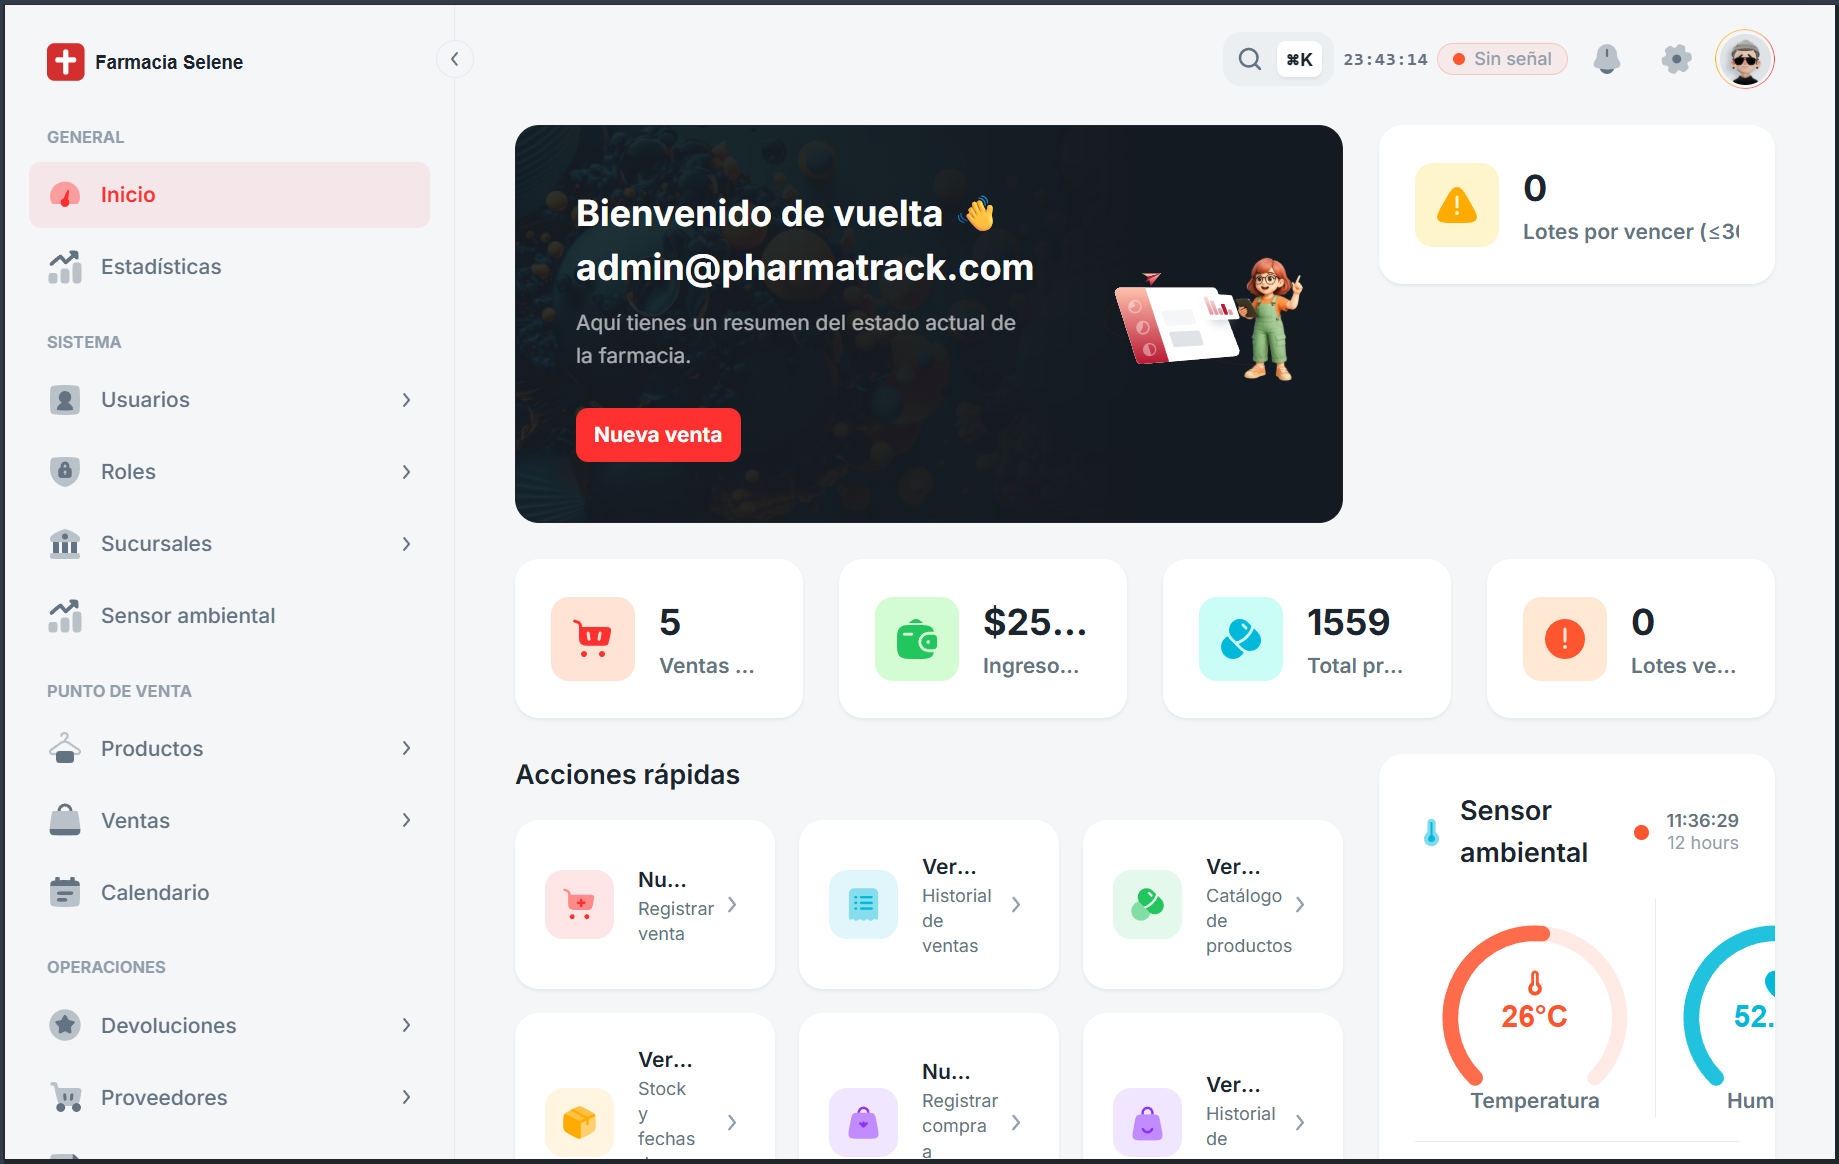
\includegraphics[width=4.0cm,height=2.4cm]{0_imagenes/Cap4/Dashboard.png}
\node[hub] (dashboard) at (5.5, 0) {%
  \textbf{\scriptsize Dashboard}%
  \nodepart{two}%
  \parbox[c][2.4cm][c]{4.0cm}{\centering\textcolor{gray!55}{\small\itshape [Dashboard.png]}}%
};

% 3. Nueva venta
% TODO: reemplazar parbox por 
\includegraphics[width=3.8cm,height=2.4cm]{0_imagenes/Cap4/NuevaVenta.png}
\node[screen] (ventas) at (11, 0) {%
  \textbf{\scriptsize Nueva venta}%
  \nodepart{two}%
  \parbox[c][2.4cm][c]{3.8cm}{\centering\textcolor{gray!50}{\small\itshape [NuevaVenta.png]}}%
};

% 4. Venta registrada
% TODO: reemplazar parbox por \includegraphics[width=3.8cm,height=2.4cm]{0_imagenes/Cap4/VentaDetalle.png}
\node[screen] (ventaok) at (16.5, 0) {%
  \textbf{\scriptsize Venta registrada}%
  \nodepart{two}%
  \parbox[c][2.4cm][c]{3.8cm}{\centering\textcolor{gray!50}{\small\itshape [VentaDetalle.png]}}%
};

% ── MÓDULOS ADICIONALES (accesibles desde el menú lateral) ───────────

% 5. Usuarios y roles
% TODO: reemplazar parbox por 
\includegraphics[width=3.8cm,height=2.4cm]{0_imagenes/Cap4/Usuarios.png}
\node[screen] (usuarios) at (1.5, -7) {%
  \textbf{\scriptsize Usuarios y roles}%
  \nodepart{two}%
  \parbox[c][2.4cm][c]{3.8cm}{\centering\textcolor{gray!50}{\small\itshape [Usuarios.png]}}%
};

% 6. Inventario
% TODO: reemplazar parbox por 
\includegraphics[width=3.8cm,height=2.4cm]{0_imagenes/Cap4/Inventario.png}
\node[screen] (inventario) at (6, -7) {%
  \textbf{\scriptsize Inventario}%
  \nodepart{two}%
  \parbox[c][2.4cm][c]{3.8cm}{\centering\textcolor{gray!50}{\small\itshape [Inventario.png]}}%
};

% 7. Compras
% TODO: reemplazar parbox por 
\includegraphics[width=3.8cm,height=2.4cm]{0_imagenes/Cap4/Compras.png}
\node[screen] (compras) at (10.5, -7) {%
  \textbf{\scriptsize Compras}%
  \nodepart{two}%
  \parbox[c][2.4cm][c]{3.8cm}{\centering\textcolor{gray!50}{\small\itshape [Compras.png]}}%
};

% 8. Sensor ambiental
% TODO: reemplazar parbox por 
\includegraphics[width=3.8cm,height=2.4cm]{0_imagenes/Cap4/Sensor.png}
\node[screen] (sensor) at (15, -7) {%
  \textbf{\scriptsize Sensor ambiental}%
  \nodepart{two}%
  \parbox[c][2.4cm][c]{3.8cm}{\centering\textcolor{gray!50}{\small\itshape [Sensor.png]}}%
};

% ── FLECHAS FLUJO PRINCIPAL ──────────────────────────────────────────

\draw[mainArrow] (login.east) -- (dashboard.west)
  node[lbl, above, midway] {acceso exitoso};

\draw[mainArrow] (dashboard.east) -- (ventas.west)
  node[lbl, above, midway] {registrar venta};

\draw[mainArrow] (ventas.east) -- (ventaok.west)
  node[lbl, above, midway] {confirmar};

% ── FLECHAS RAMIFICACIONES (menú lateral) ────────────────────────────

\coordinate (bifur) at ($(dashboard.south) + (0, -1.2)$);

\draw[branchArrow] (dashboard.south) -- (bifur)
  node[lbl, right, midway] {\itshape menú lateral};

\draw[branchArrow] (bifur) -- (usuarios.north);
\draw[branchArrow] (bifur) -- (inventario.north);
\draw[branchArrow] (bifur) -- (compras.north);
\draw[branchArrow] (bifur) -- (sensor.north);

\end{tikzpicture}%
}
\caption{Flujo de navegación del usuario en la aplicación web: la fila superior muestra el recorrido principal de registro de venta; los módulos inferiores son accesibles desde el menú lateral en cualquier momento}
\label{fig:cap4-wireflow}
\vspace{0.2cm}
\footnotesize \textbf{Fuente:} Elaboración propia.
\end{figure}

% TODO: insertar captura de pantalla del dashboard con datos reales de la farmacia
% Guardar en: 0_imagenes/Cap4/Dashboard.png
%\begin{figure}[H]
%    \centering
%    \fbox{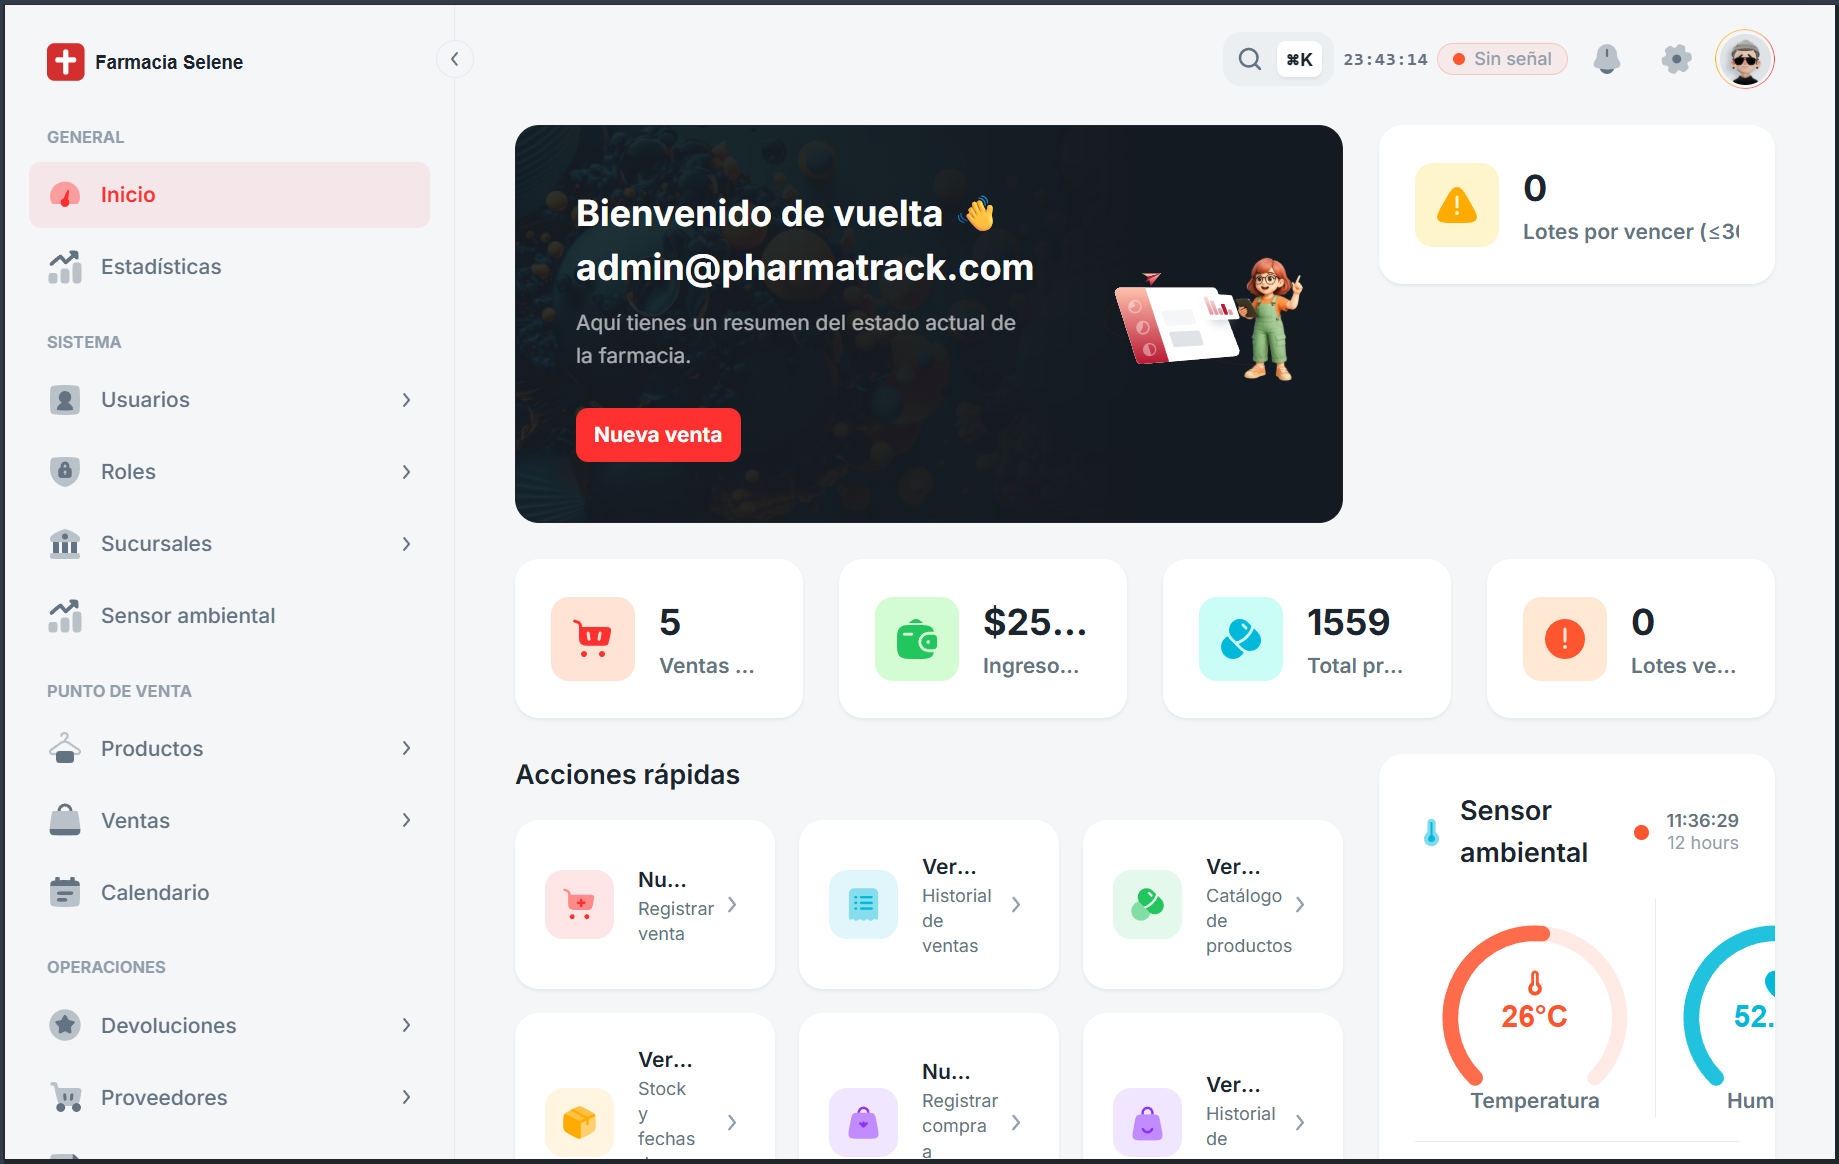
\includegraphics[width=\textwidth]{0_imagenes/Cap4/Dashboard.png}}
%    \caption{Vista del tablero principal con indicadores reales de la farmacia}
%    \label{fig:cap4-dashboard}
%    \vspace{0.2cm}
%    \footnotesize \textbf{Fuente:} Elaboración propia.
%\end{figure}

\subsection{Módulo de autenticación y control de acceso}

La integración del inicio de sesión con la API se completó en las primeras etapas del desarrollo del frontend. Durante las pruebas se identificó un comportamiento incorrecto en la visibilidad de los módulos de navegación: los elementos del menú que debían mostrarse exclusivamente al administrador aparecían para todos los usuarios, y los elementos generales quedaban ocultos. La causa era que la condición de verificación de permisos evaluaba el resultado de forma invertida —ocultaba cuando debía mostrar, y mostraba cuando debía ocultar. Una vez corregida la lógica, todos los roles visualizaron únicamente los módulos que les correspondían.

Se identificó además que una actualización de la configuración interna de la aplicación dejaba en algunos navegadores una versión desactualizada de esa configuración en memoria, lo que generaba una pantalla en blanco al recargar. El problema se resolvió versionando la configuración: al detectar una versión anterior, la aplicación la reemplaza automáticamente por la nueva.

\subsection{Módulo de productos e inventario}

El módulo de productos y el de lotes de inventario fueron los que más iteraciones requirieron durante el desarrollo. Con la propuesta inicial se lograba mostrar el listado de productos; fue necesario añadir en iteraciones sucesivas la búsqueda por nombre, los filtros por categoría y marca, la paginación de resultados, y la vista de detalle con la información del lote asociado a cada producto.

% TODO: insertar captura de pantalla del módulo de inventario/lotes con búsqueda activa
% Guardar en: 0_imagenes/Cap4/ModuloInventario.png
%\begin{figure}[H]
%    \centering
%    \fbox{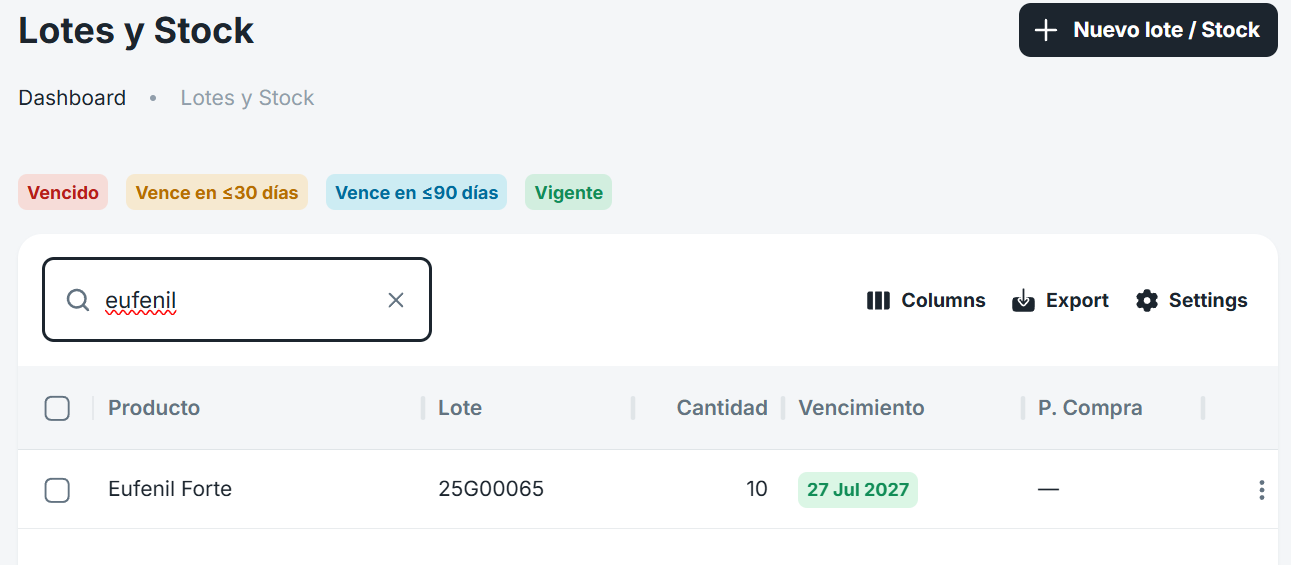
\includegraphics[width=\textwidth]{0_imagenes/Cap4/ModuloInventario.png}}
%    \caption{Módulo de inventario mostrando el listado de lotes con búsqueda y filtros activos}
%    \label{fig:cap4-inventario}
%    \vspace{0.2cm}
%    \footnotesize \textbf{Fuente:} Elaboración propia.
%\end{figure}

Un problema recurrente durante esta fase fue la desincronización entre los valores que la API enviaba y los que el frontend esperaba: cuando se modificaba un conjunto de opciones válidas en la API —por ejemplo, los estados posibles de un lote o los tipos de movimiento— la interfaz seguía usando los valores anteriores, generando errores en los formularios. Esto se corrigió estableciendo un proceso de revisión explícita de estos valores cada vez que se actualizaba la API.

\subsection{Módulo de ventas y lector de código de barras}

El módulo de ventas fue el de mayor complejidad en el frontend: el formulario de registro de venta pasó por once versiones a lo largo del desarrollo. Con la versión inicial se podía seleccionar productos y registrar el encabezado de la venta; en iteraciones posteriores se incorporó el seguimiento por lote, la sección de pagos con soporte para múltiples métodos, la creación de lotes directamente desde el formulario, y finalmente el modo lector de código de barras.

El modo lector —que se activa con la tecla \textbf{F2} y redirige el foco al campo de escaneo— funcionó correctamente desde las primeras pruebas con productos reales de la farmacia. Los ajustes que requirió fueron de carácter visual: se añadió un banner animado en la parte superior del formulario para indicar que el modo está activo, y un indicador flotante que confirma visualmente si el código escaneado fue reconocido o no.

Durante las pruebas del formulario de pago se identificó que al escribir el monto en el campo correspondiente, el número se concatenaba con el cero inicial del campo en lugar de reemplazarlo, generando valores incorrectos. El comportamiento se corrigió haciendo que el campo seleccione todo su contenido automáticamente al recibir el foco, de modo que el primer dígito tecleado sustituya el valor anterior.

% TODO: insertar captura de pantalla del formulario de venta con el modo lector activo (banner F2)
% Guardar en: 0_imagenes/Cap4/ModoLector.png
%\begin{figure}[H]
%    \centering
%    \fbox{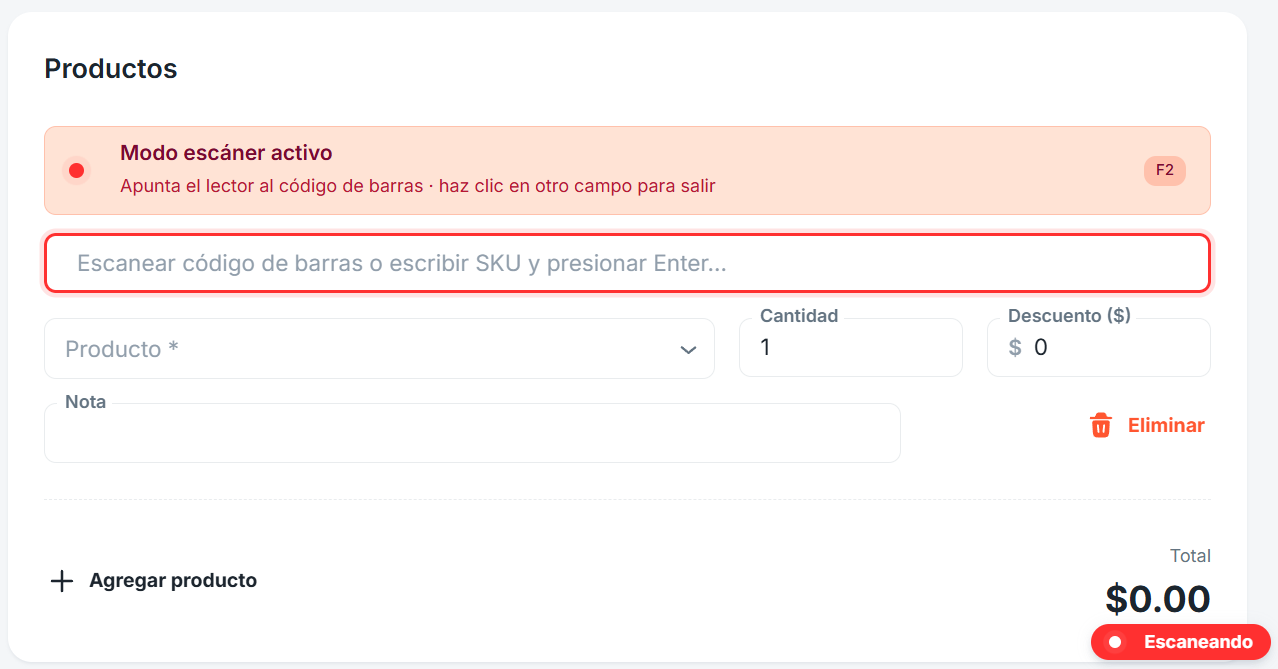
\includegraphics[width=\textwidth]{0_imagenes/Cap4/ModoLector.png}}
%    \caption{Formulario de registro de venta con el modo lector de código de barras activo}
%    \label{fig:cap4-modo-lector}
%    \vspace{0.2cm}
%    \footnotesize \textbf{Fuente:} Elaboración propia.
%\end{figure}

\subsection{Tablero de indicadores y monitoreo del sensor}

El tablero principal se construyó inicialmente con datos simulados para validar la disposición visual de los indicadores. Una vez que los módulos de ventas, inventario y sensor estuvieron operativos en la API, se realizó la conexión con datos reales: el tablero pasó a mostrar el total de ventas del día, el nivel de existencias, las alertas de lotes próximos a vencer y las lecturas actuales de temperatura y humedad del nodo sensor.

Durante esta conexión se identificó que el tablero realizaba tres llamadas independientes a la API al cargar —una por cada grupo de indicadores— lo que generaba una demora visible al abrir la vista. Para resolver esto se consolidó la información en un único punto de la API que devuelve todos los indicadores en una sola respuesta, reduciendo el tiempo de carga del tablero de forma notoria.

% TODO: insertar captura de pantalla del módulo de monitoreo del sensor con lecturas en tiempo real
% Guardar en: 0_imagenes/Cap4/MonitorSensor.png
%\begin{figure}[H]
%    \centering
%    \fbox{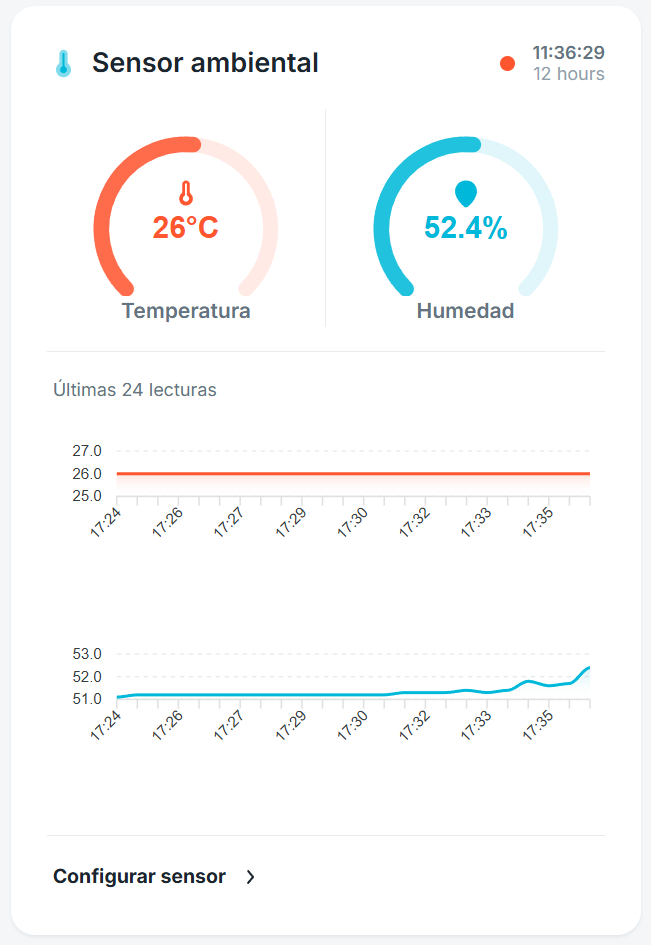
\includegraphics[width=0.9\textwidth]{0_imagenes/Cap4/MonitorSensor.png}}
%    \caption{Módulo de monitoreo ambiental mostrando lecturas de temperatura y humedad del nodo sensor}
%    \label{fig:cap4-sensor-monitor}
%    \vspace{0.2cm}
%    \footnotesize \textbf{Fuente:} Elaboración propia.
%\end{figure}

\subsection{Correcciones identificadas durante las pruebas}

\begin{longtable}{|p{3.2cm}|p{4.0cm}|p{7.3cm}|}

\caption{Correcciones realizadas a la interfaz web durante las pruebas} \label{tab:cap4-front-correcciones} \\

\hline
\rowcolor{gray!20}
\textbf{Módulo} & \textbf{Problema identificado} & \textbf{Corrección aplicada} \\
\hline
\endfirsthead

\hline
\rowcolor{gray!20}
\textbf{Módulo} & \textbf{Problema identificado} & \textbf{Corrección aplicada} \\
\hline
\endhead

\hline
\multicolumn{3}{|r|}{\small Continúa en la siguiente página} \\
\hline
\endfoot

\hline
\endlastfoot

Visibilidad de módulos &
La lógica de verificación de permisos estaba invertida: ocultaba lo que debía mostrarse y mostraba lo que debía ocultarse &
Se corrigió la condición de verificación; cada rol visualiza únicamente los módulos que le corresponden \\
\hline

Pantalla en blanco &
Una actualización de la configuración interna dejaba versiones desactualizadas en el navegador, causando pantalla en blanco al recargar &
Se versionó la configuración para forzar su actualización automática al detectar una versión anterior \\
\hline

Enrutamiento en Vercel &
Al acceder directamente a una ruta o recargar la página, Vercel devolvía un error 404 porque no encontraba el archivo correspondiente &
Se añadió una regla de redirección que redirige cualquier URL al punto de entrada de la aplicación \\
\hline

Tipos de datos entre sistemas &
Cuando la API modificaba sus conjuntos de valores válidos, la interfaz seguía usando los valores anteriores, generando errores en los formularios &
Se estableció una revisión de estos valores en cada actualización de la API \\
\hline

Límite de solicitudes &
El servidor rechazaba solicitudes frecuentes con un error de límite de tasa, y la interfaz no lo manejaba, dejando al usuario sin respuesta &
Se añadió un reintento automático que respeta el tiempo de espera indicado por el servidor antes de reintentar \\
\hline

Formulario de pago &
Al escribir el monto en el campo de pago, el número se concatenaba con el valor inicial del campo en lugar de reemplazarlo &
Se configuró el campo para seleccionar su contenido al recibir el foco, de modo que el primer dígito sustituya el valor anterior \\

\end{longtable}
\vspace{0.1cm}
{\footnotesize \textbf{Fuente:} Elaboración propia.}

\subsection{Resultados}

Al finalizar las pruebas, los dieciséis módulos de navegación de la interfaz operan de forma correcta contra la API de producción. El flujo completo de una venta —desde la apertura del formulario hasta la confirmación, incluyendo el escaneo de códigos de barras y el registro del pago— se completó de forma exitosa en las pruebas con productos reales de la farmacia. El tablero de indicadores muestra datos actualizados en tiempo real y las lecturas del nodo sensor se visualizan correctamente en el módulo de monitoreo.

% =============================================
% SECCIÓN 4.4: NODO SENSOR ESP32
% =============================================

\clearpage
\section{Pruebas del nodo sensor}

Las pruebas del nodo sensor cubrieron tres aspectos: la correcta transmisión de las lecturas al servidor, el comportamiento del firmware ante valores fuera de rango, y la estabilidad de la conexión WiFi. Las pruebas se realizaron en el entorno de desarrollo mientras se finaliza el diseño del gabinete físico para la instalación en la farmacia.

\subsection{Transmisión de datos al servidor}

Con la versión inicial del firmware el nodo realizaba lecturas del sensor AHT10 cada 30 segundos y las enviaba al servidor de la API. Al revisar el tablero de la aplicación web se observó que no aparecían nuevas lecturas, a pesar de que el nodo indicaba en su salida de diagnóstico que las solicitudes se enviaban correctamente.

La causa del problema fue una barra inclinada adicional al final de la dirección del servidor configurada en el firmware. Al recibir una solicitud con esa barra, el servidor respondía con un error de ruta no encontrada en lugar de procesar el dato. Una vez eliminada la barra de la dirección, las lecturas comenzaron a registrarse correctamente en la base de datos y a aparecer en el tablero en tiempo real.

% TODO: insertar captura de pantalla de la salida serial del ESP32 mostrando lecturas enviadas correctamente
% Guardar en: 0_imagenes/Cap4/SensorSerial.png
%\begin{figure}[H]
%    \centering
%    \fbox{\includegraphics[width=0.85\textwidth]{0_imagenes/Cap4/SensorSerial.png}}
%    \caption{Salida de diagnóstico del nodo sensor mostrando lecturas enviadas al servidor}
%    \label{fig:cap4-serial}
%    \vspace{0.2cm}
%    \footnotesize \textbf{Fuente:} Elaboración propia.
%\end{figure}

\subsection{Incidente de hardware: conflicto de pines}

Durante las pruebas de ensamble se intentó apagar el LED RGB integrado en la placa del ESP32-C5 para que no emitiera luz durante la operación normal del nodo. Al implementar el control del LED por software se comenzaron a registrar lecturas erráticas del sensor AHT10: valores de temperatura y humedad inconsistentes que el firmware descartaba por estar fuera del rango de validación.

La investigación del problema reveló que el pin del microcontrolador asignado al LED RGB coincidía con el mismo pin utilizado como línea de datos del bus de comunicación con el sensor AHT10. Al intentar controlar el LED, el firmware generaba señales que interferían con la comunicación del sensor, corrompiendo las lecturas. La figura siguiente ilustra el conflicto:

\begin{figure}[H]
\centering
\begin{tikzpicture}[font=\small]

% Chip ESP32-C5
\draw[thick, rounded corners=5pt, fill=gray!8]
    (-1.8, -2.4) rectangle (1.8, 2.4);
\node[font=\small\bfseries] at (0, 2.0) {ESP32-C5};

% Pin GPIO 8 en el chip
\draw[thick] (1.8, 0.4) -- (2.6, 0.4);
\fill[gray!50] (2.3, 0.15) rectangle (2.6, 0.65);
\node[anchor=east, font=\scriptsize] at (1.75, 0.4) {GPIO 8};

% Bifurcación del pin
\draw[thick] (2.6, 0.4) -- (3.4, 0.4);
\draw[thick] (3.4, 0.4) -- (3.4,  1.6);
\draw[thick] (3.4, 0.4) -- (3.4, -0.8);

% Destino 1: AHT10 (uso correcto)
\draw[-{Stealth}, thick] (3.4, 1.6) -- (5.0, 1.6);
\draw[thick, rounded corners=3pt, fill=gray!10]
    (5.0, 1.15) rectangle (9.2, 2.05);
\node[anchor=west, font=\scriptsize] at (5.15, 1.72) {\textbf{Sensor AHT10}};
\node[anchor=west, font=\scriptsize, text=gray!60] at (5.15, 1.32) {SDA — bus I\textsuperscript{2}C};

% Destino 2: LED RGB (conflicto)
\draw[-{Stealth}, thick, dashed] (3.4, -0.8) -- (5.0, -0.8);
\draw[thick, rounded corners=3pt, fill=gray!10, dashed]
    (5.0, -1.25) rectangle (9.2, -0.35);
\node[anchor=west, font=\scriptsize] at (5.15, -0.52) {\textbf{LED RGB integrado}};
\node[anchor=west, font=\scriptsize, text=gray!60] at (5.15, -0.92) {RGB\_PIN (placa)};

% Símbolo de conflicto en la bifurcación
\node[circle, draw, thick, fill=white, minimum size=0.7cm,
      font=\small\bfseries] at (3.4, 0.4) {!};

% Etiqueta de conflicto
\node[font=\scriptsize, text=gray!70, align=center] at (3.4, -1.75)
    {Mismo pin:\\dos funciones};

% Resultado: interferencia
\draw[-{Stealth}, thick, gray!50] (9.2, 1.6) -- (10.4, 1.6) -- (10.4, -0.1);
\draw[-{Stealth}, thick, gray!50] (9.2, -0.8) -- (10.4, -0.8) -- (10.4, -0.1);
\draw[thick, rounded corners=3pt, fill=gray!20]
    (10.4, -0.55) rectangle (13.2, 0.35);
\node[font=\scriptsize, align=center] at (11.8, -0.1)
    {Interferencia:\\lecturas erróneas};

\end{tikzpicture}
\caption{Conflicto de pines detectado durante las pruebas: GPIO 8 estaba asignado simultáneamente a la línea de datos del sensor AHT10 y al control del LED RGB, causando interferencia en las lecturas}
\label{fig:cap4-pin-conflicto}
\vspace{0.2cm}
\footnotesize \textbf{Fuente:} Elaboración propia.
\end{figure}

Dado que la documentación técnica de esa revisión de la placa no especificaba el pin correcto del LED, no fue posible resolver el conflicto por software. La solución fue retirar físicamente el LED de la placa mediante soldadura y eliminar todo el código relacionado del firmware. Tras esta intervención el sensor recuperó su comportamiento normal y las lecturas se transmitieron sin interrupciones.

% TODO: insertar fotografía del nodo sensor ensamblado (ESP32 + AHT10 + cables)
% Guardar en: 0_imagenes/Cap4/NodoEnsamblado.jpg
%\begin{figure}[H]
%    \centering
%    \fbox{\includegraphics[width=0.70\textwidth]{0_imagenes/Cap4/NodoEnsamblado.jpg}}
%    \caption{Nodo sensor ensamblado: ESP32-C5 con el sensor AHT10 conectado por bus I\textsuperscript{2}C}
%    \label{fig:cap4-nodo}
%    \vspace{0.2cm}
%    \footnotesize \textbf{Fuente:} Elaboración propia.
%\end{figure}

\subsection{Validación de lecturas fuera de rango}

El firmware descarta automáticamente cualquier lectura que caiga fuera de los rangos físicamente plausibles definidos para el sensor: entre $-10\,^\circ\text{C}$ y $85\,^\circ\text{C}$ para temperatura, y entre $0\,\%$ y $100\,\%$ para humedad relativa. Estos límites son deliberadamente amplios respecto a las condiciones normales de una farmacia —donde los rangos de operación son mucho más estrechos— con el objetivo de filtrar únicamente lecturas claramente erróneas sin descartar valores extremos que pudieran ser reales en una situación de emergencia.

Se verificó este comportamiento forzando manualmente valores fuera de rango en el entorno de pruebas: el firmware los identificó correctamente y los descartó sin enviarlos al servidor, registrando el descarte en la salida de diagnóstico.

\begin{figure}[H]
\centering
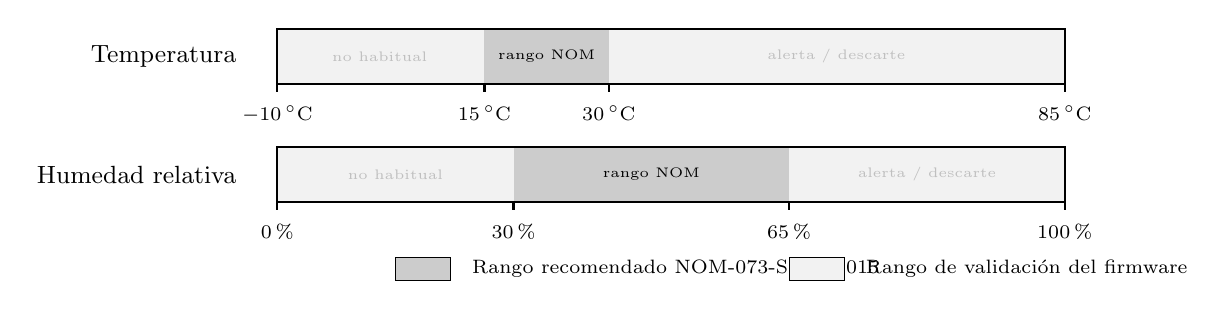
\begin{tikzpicture}[font=\scriptsize]

% ── Temperatura ───────────────────────────────────────────────
\node[anchor=east, font=\small] at (-0.4, 1.0) {Temperatura};

% Barra completa: -10°C a 85°C = 95°C → escala 10cm/95°C ≈ 0.1053 cm/°C
% Posiciones (x=0 → -10°C): 15°C→2.63, 30°C→4.21, 85°C→10.0
\fill[gray!10]  (0,    0.65) rectangle (10.0, 1.35);  % rango firmware (fondo)
\fill[gray!40]  (2.63, 0.65) rectangle (4.21, 1.35);  % rango NOM (15–30°C)
\draw[thick]    (0,    0.65) rectangle (10.0, 1.35);

% Etiquetas de límites
\draw[thick] (0,    0.55) -- (0,    0.65);
\draw[thick] (2.63, 0.55) -- (2.63, 0.65);
\draw[thick] (4.21, 0.55) -- (4.21, 0.65);
\draw[thick] (10.0, 0.55) -- (10.0, 0.65);
\node[anchor=north] at (0,    0.50) {$-10\,^\circ$C};
\node[anchor=north] at (2.63, 0.50) {$15\,^\circ$C};
\node[anchor=north] at (4.21, 0.50) {$30\,^\circ$C};
\node[anchor=north] at (10.0, 0.50) {$85\,^\circ$C};

% Anotaciones internas
\node[font=\tiny, text=gray!50] at (1.3,  1.0) {no habitual};
\node[font=\tiny]               at (3.42, 1.0) {rango NOM};
\node[font=\tiny, text=gray!50] at (7.1,  1.0) {alerta / descarte};

% ── Humedad ───────────────────────────────────────────────────
\node[anchor=east, font=\small] at (-0.4, -0.5) {Humedad relativa};

% Barra: 0% a 100% → 10cm / 100% = 0.10 cm/%
% 30%→3.0, 65%→6.5
\fill[gray!10]  (0,   -0.85) rectangle (10.0, -0.15);
\fill[gray!40]  (3.0, -0.85) rectangle (6.5,  -0.15);
\draw[thick]    (0,   -0.85) rectangle (10.0, -0.15);

\draw[thick] (0,   -0.95) -- (0,   -0.85);
\draw[thick] (3.0, -0.95) -- (3.0, -0.85);
\draw[thick] (6.5, -0.95) -- (6.5, -0.85);
\draw[thick] (10.0,-0.95) -- (10.0,-0.85);
\node[anchor=north] at (0,    -1.0) {$0\,\%$};
\node[anchor=north] at (3.0,  -1.0) {$30\,\%$};
\node[anchor=north] at (6.5,  -1.0) {$65\,\%$};
\node[anchor=north] at (10.0, -1.0) {$100\,\%$};

\node[font=\tiny, text=gray!50] at (1.5,  -0.5) {no habitual};
\node[font=\tiny]               at (4.75, -0.5) {rango NOM};
\node[font=\tiny, text=gray!50] at (8.25, -0.5) {alerta / descarte};

% ── Leyenda ───────────────────────────────────────────────────
\fill[gray!40] (1.5, -1.85) rectangle (2.2, -1.55);
\draw          (1.5, -1.85) rectangle (2.2, -1.55);
\node[anchor=west, font=\scriptsize] at (2.35, -1.70)
    {Rango recomendado NOM-073-SSA1-2015};

\fill[gray!10] (6.5, -1.85) rectangle (7.2, -1.55);
\draw          (6.5, -1.85) rectangle (7.2, -1.55);
\node[anchor=west, font=\scriptsize] at (7.35, -1.70)
    {Rango de validación del firmware};

\end{tikzpicture}
\caption{Rangos de validación del firmware en comparación con los rangos recomendados por la NOM-073-SSA1-2015: el firmware descarta lecturas fuera de los límites del hardware; las alertas se generan al superar los umbrales de la norma}
\label{fig:cap4-rangos}
\vspace{0.2cm}
\footnotesize \textbf{Fuente:} Elaboración propia.
\end{figure}

\subsection{Resultados}

Resuelto el conflicto de pines y corregida la dirección del servidor, el nodo operó de forma estable durante las sesiones de prueba: las lecturas se transmitieron correctamente cada 30 segundos y aparecieron en el tablero de la aplicación web sin interrupciones. Las pruebas de operación continua en la farmacia quedan pendientes hasta que se concluya el rediseño del gabinete físico descrito en la sección siguiente.

% =============================================
% SECCIÓN 4.5: GABINETE E INTEGRACIÓN
% =============================================

\clearpage
\section{Pruebas del gabinete y lector de código de barras}

\subsection{Gabinete impreso en 3D}

Con el primer diseño del gabinete se utilizaron las dimensiones nominales de cada componente tal como las especifican los fabricantes: el largo, ancho y alto de la placa del ESP32-C5, el módulo del sensor AHT10 y las pantallas OLED. Las piezas se modelaron con esas medidas y se fabricaron mediante impresión 3D.

Al intentar montar los componentes dentro del gabinete se identificó que no era posible alojarlos correctamente: los conectores Dupont —los terminales de los cables que unen el microcontrolador con el sensor— sobresalen varios milímetros por encima de la superficie de la placa, una dimensión que las especificaciones del fabricante no incluyen. Este sobredimensionamiento vertical impidió cerrar el gabinete sin ejercer presión sobre los cables, lo que representaba un riesgo para las conexiones.

% TODO: insertar fotografía del primer gabinete impreso mostrando el problema de espacio
% Guardar en: 0_imagenes/Cap4/GabineteV1.jpg
%\begin{figure}[H]
%    \centering
%    \fbox{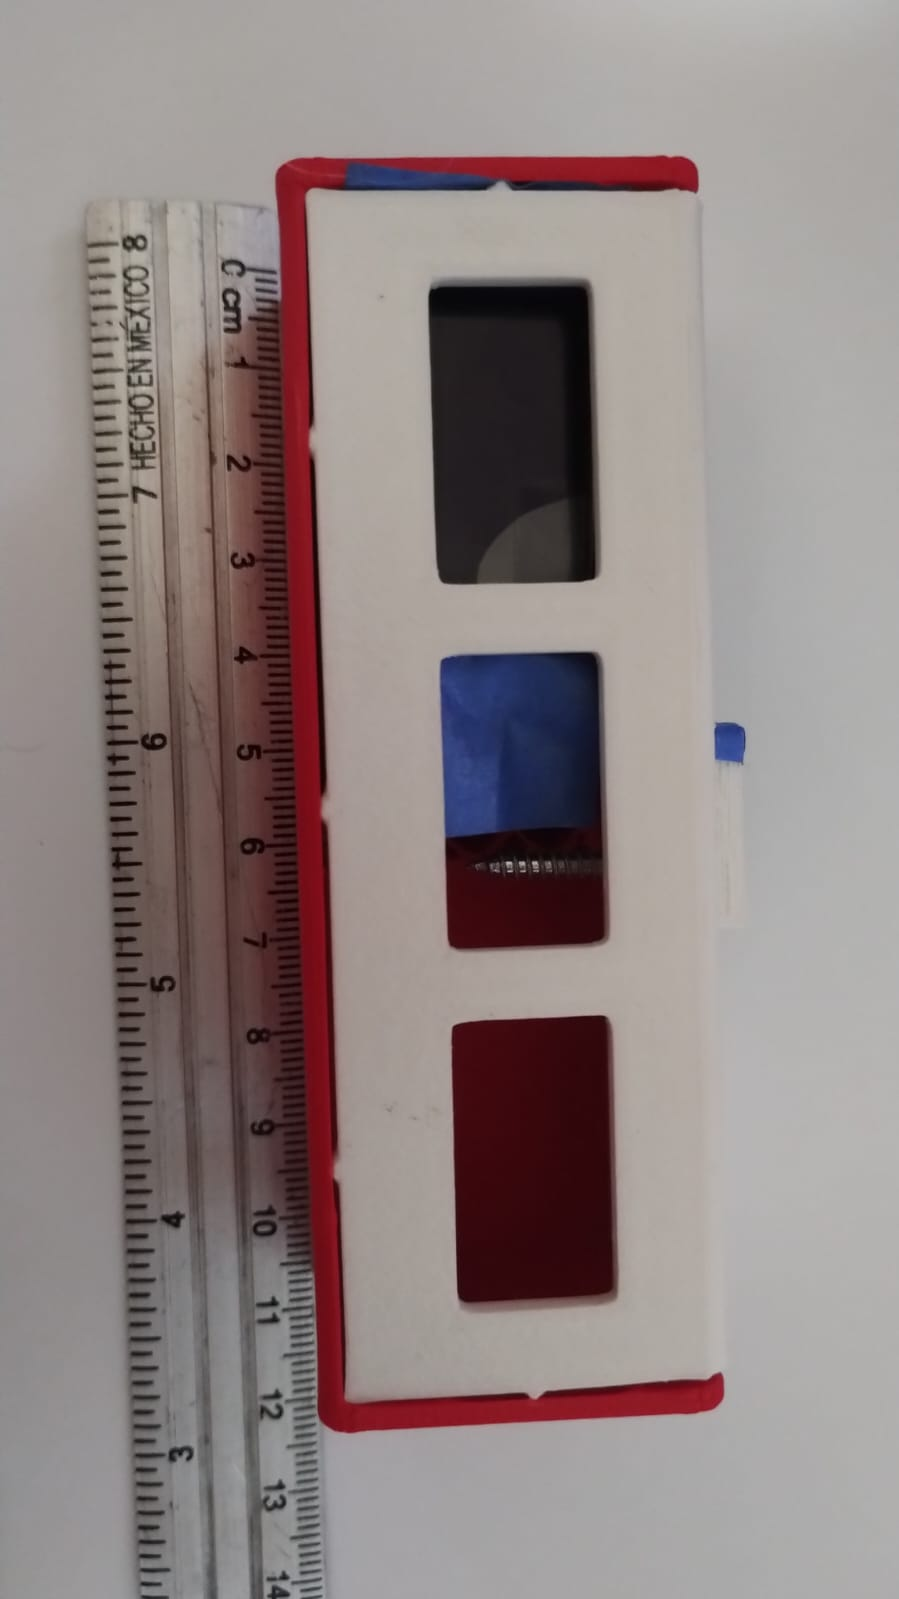
\includegraphics[width=0.70\textwidth]{0_imagenes/Cap4/GabineteV1.jpg}}
%    \caption{Primer diseño del gabinete: los conectores sobresalen e impiden el cierre correcto}
%    \label{fig:cap4-gabinete-v1}
%    \vspace{0.2cm}
%    \footnotesize \textbf{Fuente:} Elaboración propia.
%\end{figure}

\begin{figure}[H]
\centering
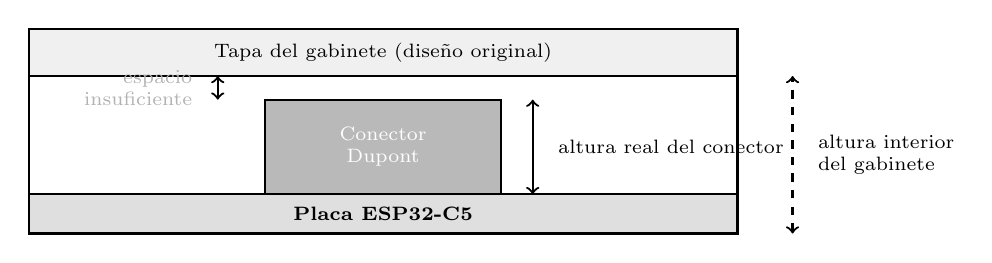
\begin{tikzpicture}[font=\small]

% ── PCB ───────────────────────────────────────────────────────
\fill[gray!25] (0, 0) rectangle (9.0, 0.5);
\draw[thick]   (0, 0) rectangle (9.0, 0.5);
\node[font=\scriptsize\bfseries] at (4.5, 0.25) {Placa ESP32-C5};

% ── Conector Dupont (sobresale de la placa) ───────────────────
\fill[gray!55] (3.0, 0.5) rectangle (6.0, 1.7);
\draw[thick]   (3.0, 0.5) rectangle (6.0, 1.7);
\node[font=\scriptsize, text=white, align=center] at (4.5, 1.1)
    {Conector\\Dupont};

% ── Tapa del gabinete (altura diseñada — insuficiente) ────────
\fill[gray!12] (0, 2.0) rectangle (9.0, 2.6);
\draw[thick]   (0, 2.0) rectangle (9.0, 2.6);
\node[font=\scriptsize] at (4.5, 2.3) {Tapa del gabinete (diseño original)};

% ── Paredes laterales del gabinete ───────────────────────────
\draw[thick] (0, 0) -- (0, 2.6);
\draw[thick] (9.0, 0) -- (9.0, 2.6);

% ── Flecha: altura real del conector ─────────────────────────
\draw[<->, thick] (6.4, 0.5) -- (6.4, 1.7);
\node[anchor=west, font=\scriptsize] at (6.6, 1.1)
    {altura real del conector};

% ── Flecha: espacio disponible (insuficiente) ─────────────────
\draw[<->, thick] (2.4, 1.7) -- (2.4, 2.0);
\node[anchor=east, font=\scriptsize, text=gray!60, align=right]
    at (2.2, 1.85) {espacio\\insuficiente};

% ── Flecha: altura interior total del gabinete ───────────────
\draw[<->, thick, dashed] (9.7, 0) -- (9.7, 2.0);
\node[anchor=west, font=\scriptsize, align=left] at (9.9, 1.0)
    {altura interior\\del gabinete};

\end{tikzpicture}
\caption{Vista lateral esquemática del gabinete original: la altura del conector Dupont supera el espacio interior disponible, impidiendo cerrar la tapa sin comprimir los cables}
\label{fig:cap4-gabinete-problema}
\vspace{0.2cm}
\footnotesize \textbf{Fuente:} Elaboración propia.
\end{figure}

Para resolver esto fue necesario relevar manualmente las dimensiones reales del conjunto ensamblado —incluyendo los conectores y el radio de curvatura de los cables— y rediseñar el gabinete con esas medidas. El rediseño está actualmente en proceso; la nueva versión contempla una altura interior mayor en la base para dar espacio a los conectores y una distribución diferente de los componentes para reducir el recorrido de los cables internos.

% TODO: insertar imagen del modelo 3D del gabinete rediseñado (captura del software de modelado)
% Guardar en: 0_imagenes/Cap4/GabineteV2Modelo.png
%\begin{figure}[H]
%    \centering
%    \fbox{\includegraphics[width=0.70\textwidth]{0_imagenes/Cap4/GabineteV2Modelo.png}}
%    \caption{Modelo del gabinete rediseñado con espacio adicional para conectores}
%    \label{fig:cap4-gabinete-v2}
%    \vspace{0.2cm}
%    \footnotesize \textbf{Fuente:} Elaboración propia.
%\end{figure}

\subsection{Lector de código de barras}

El lector de código de barras se conectó al equipo de cómputo de la farmacia mediante USB y fue reconocido automáticamente por el sistema operativo como un dispositivo de teclado estándar, sin requerir la instalación de controladores adicionales. Se realizaron pruebas de escaneo con productos reales del inventario de la farmacia: todos los códigos de barras presentes en los productos fueron leídos correctamente y el código obtenido coincidió con el registrado en el catálogo del sistema.

% TODO: insertar fotografía del lector de código de barras escaneando un producto real de la farmacia
% Guardar en: 0_imagenes/Cap4/LectorEnUso.jpg
%\begin{figure}[H]
%    \centering
%    \fbox{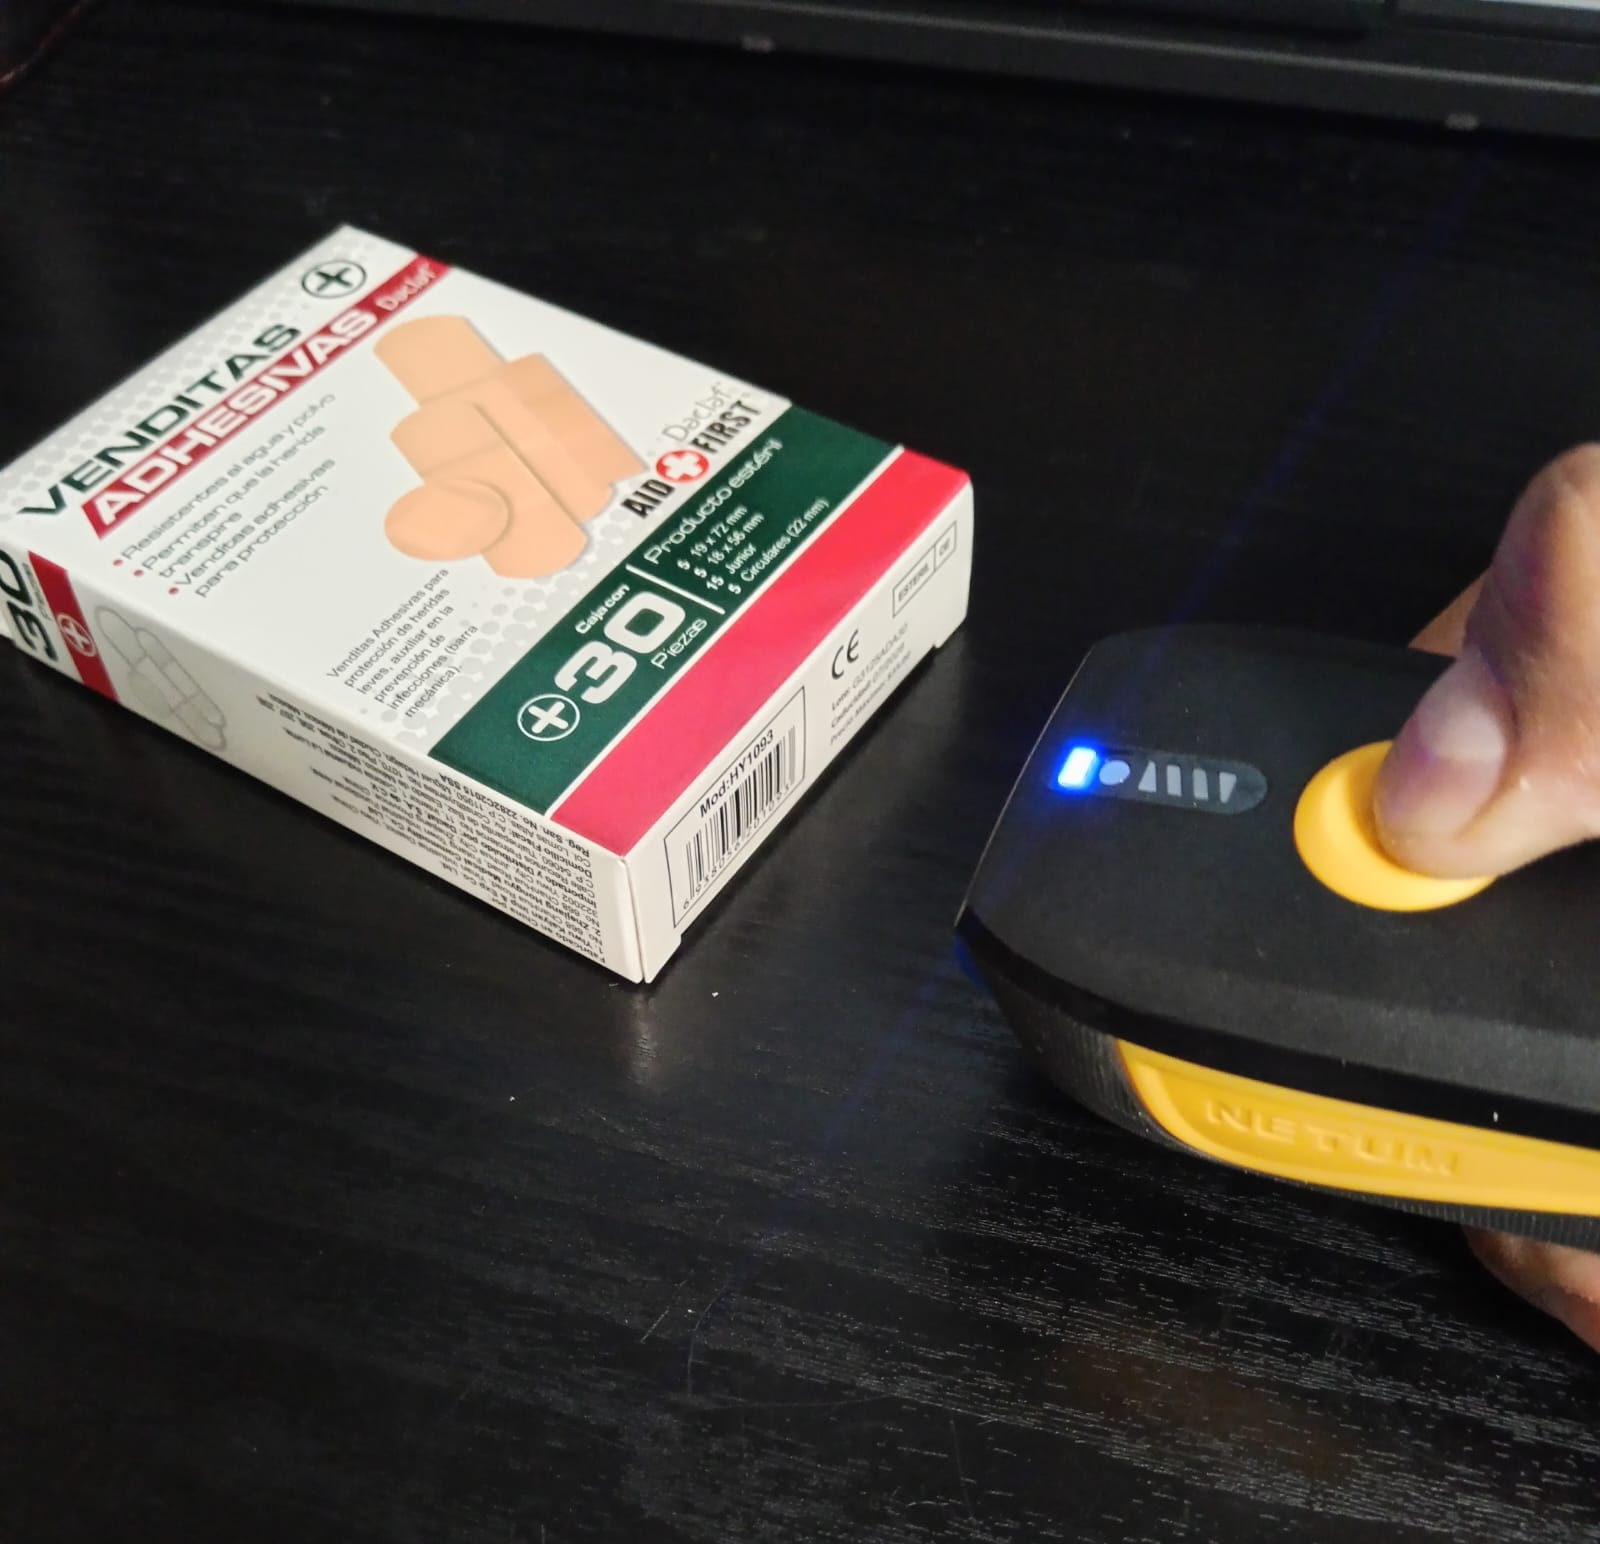
\includegraphics[width=0.70\textwidth]{0_imagenes/Cap4/LectorEnUso.jpg}}
%    \caption{Lector de código de barras en uso con un producto real de la farmacia}
%    \label{fig:cap4-lector-uso}
%    \vspace{0.2cm}
%    \footnotesize \textbf{Fuente:} Elaboración propia.
%\end{figure}

La integración del lector con el flujo de registro de ventas en la interfaz web —incluyendo la activación del modo de escaneo, la búsqueda en el catálogo local y la confirmación visual del resultado— se describió en la sección 4.3 de este capítulo.

% =============================================
% SECCIÓN 4.6: INTEGRACIÓN DEL SISTEMA
% =============================================

\clearpage
\section{Prueba de integración del sistema}

Una vez verificados los componentes de forma individual, se realizó una prueba de integración del sistema completo para confirmar que los cinco objetivos específicos operan de forma conjunta. El escenario de prueba cubrió el flujo de extremo a extremo más representativo del sistema: desde la medición ambiental del nodo sensor hasta el registro de una venta con descuento de inventario, pasando por todas las capas del sistema.

\begin{figure}[H]
\centering
\begin{tikzpicture}[font=\small,
    comp/.style={rectangle, draw, rounded corners=4pt,
                 minimum width=3.0cm, minimum height=1.0cm,
                 align=center, fill=gray!8},
    arr/.style={-{Stealth}, thick}
]

% Componentes
\node[comp] (sensor) at (0,    0) {\textbf{Nodo sensor}\\{\scriptsize ESP32 + AHT10}};
\node[comp] (api)    at (5.2,  0) {\textbf{API REST}\\{\scriptsize Railway}};
\node[comp] (db)     at (5.2, -2.2) {\textbf{Base de datos}\\{\scriptsize PostgreSQL}};
\node[comp] (web)    at (10.4,  0) {\textbf{Interfaz web}\\{\scriptsize Vercel}};
\node[comp] (user)   at (10.4, -2.2) {\textbf{Usuario}\\{\scriptsize navegador}};

% Flujo sensor → API
\draw[arr] (sensor.east) -- node[above, font=\scriptsize]{HTTPS POST} (api.west);

% Flujo API ↔ DB
\draw[arr] (api.south) -- node[right, font=\scriptsize]{guarda} (db.north);

% Flujo web → API
\draw[arr] (web.west) -- node[above, font=\scriptsize]{consultas} (api.east);

% Flujo API → web (respuesta)
\draw[arr] ([yshift=-0.25cm]api.east) --
    node[below, font=\scriptsize]{datos} ([yshift=-0.25cm]web.west);

% Flujo usuario ↔ web
\draw[arr] (user.north) -- node[right, font=\scriptsize]{opera} (web.south);

% Etiquetas de resultado
\node[font=\scriptsize, text=gray!60, align=center] at (2.6, 0.55)
    {lectura cada\\30 segundos};
\node[font=\scriptsize, text=gray!60, align=center] at (7.8, 0.55)
    {tablero, ventas,\\alertas};

\end{tikzpicture}
\caption{Flujo de integración del sistema completo: el nodo sensor envía lecturas a la API, que las almacena en la base de datos; la interfaz web consulta la API para mostrar los datos al usuario}
\label{fig:cap4-integracion}
\vspace{0.2cm}
\footnotesize \textbf{Fuente:} Elaboración propia.
\end{figure}

La prueba confirmó que el flujo opera correctamente de extremo a extremo: el nodo sensor transmite las lecturas ambientales al servidor cada 30 segundos, la API las almacena en la base de datos y la interfaz web las muestra en el módulo de monitoreo sin intervención adicional. De forma simultánea, el registro de ventas con descuento de inventario por lote, la autenticación por roles y la navegación por módulos funcionaron de forma conjunta sin conflictos entre componentes.

% TODO: insertar captura de pantalla del dashboard mostrando lecturas del sensor y datos de ventas
%       simultáneamente — es la evidencia visual más directa de que el sistema integrado funciona
% Guardar en: 0_imagenes/Cap4/SistemaIntegrado.png
%\begin{figure}[H]
%    \centering
%    \fbox{\includegraphics[width=\textwidth]{0_imagenes/Cap4/SistemaIntegrado.png}}
%    \caption{Tablero principal mostrando simultáneamente indicadores de ventas e inventario y
%             lecturas en tiempo real del nodo sensor, evidencia de la operación integrada del sistema}
%    \label{fig:cap4-sistema-integrado}
%    \vspace{0.2cm}
%    \footnotesize \textbf{Fuente:} Elaboración propia.
%\end{figure}

Los elementos pendientes de integración al momento de la redacción de este capítulo son las pantallas OLED del nodo sensor —en espera del rediseño del gabinete— y las pruebas de operación continua del sistema en las instalaciones de la farmacia, previstas para realizarse una vez que el gabinete esté concluido.
